%!TEX TS-program = xelatex
%!TEX encoding = UTF-8 Unicode
% Awesome CV LaTeX Template for CV/Resume
%
% This template has been downloaded from:
% https://github.com/posquit0/Awesome-CV
%
% Author:
% Claud D. Park <posquit0.bj@gmail.com>
% http://www.posquit0.com
%
%
% Adapted to be an Rmarkdown template by Mitchell O'Hara-Wild
% 23 November 2018
%
% Template license:
% CC BY-SA 4.0 (https://creativecommons.org/licenses/by-sa/4.0/)
%
%-------------------------------------------------------------------------------
% CONFIGURATIONS
%-------------------------------------------------------------------------------
% A4 paper size by default, use 'letterpaper' for US letter
\documentclass[11pt,a4paper,]{awesome-cv}

% Configure page margins with geometry
\usepackage{geometry}
\geometry{left=1.4cm, top=.8cm, right=1.4cm, bottom=1.8cm, footskip=.5cm}


% Specify the location of the included fonts
\fontdir[fonts/]

% Color for highlights
% Awesome Colors: awesome-emerald, awesome-skyblue, awesome-red, awesome-pink, awesome-orange
%                 awesome-nephritis, awesome-concrete, awesome-darknight

\definecolor{awesome}{HTML}{207373}

% Colors for text
% Uncomment if you would like to specify your own color
% \definecolor{darktext}{HTML}{414141}
% \definecolor{text}{HTML}{333333}
% \definecolor{graytext}{HTML}{5D5D5D}
% \definecolor{lighttext}{HTML}{999999}

% Set false if you don't want to highlight section with awesome color
\setbool{acvSectionColorHighlight}{true}

% If you would like to change the social information separator from a pipe (|) to something else
\renewcommand{\acvHeaderSocialSep}{\quad\textbar\quad}

\def\endfirstpage{\newpage}

%-------------------------------------------------------------------------------
%	PERSONAL INFORMATION
%	Comment any of the lines below if they are not required
%-------------------------------------------------------------------------------
% Available options: circle|rectangle,edge/noedge,left/right

\photo{../images/JDL.jpg}
\name{Juan David}{Leongómez}

\position{Profesor Asociado}
\address{Facultad de Psicología, Universidad El Bosque}

\mobile{(+57) 601-6489000 Ext. 1901}
\email{\href{mailto:jleongomez@unbosque.edu.co}{\nolinkurl{jleongomez@unbosque.edu.co}}}
\homepage{jdleongomez.info/es}
\orcid{0000-0002-0092-6298}

% \gitlab{gitlab-id}
% \stackoverflow{SO-id}{SO-name}
% \skype{skype-id}
% \reddit{reddit-id}

\quote{Soy un investigador interesado principalmente en el
comportamiento humano, así como en los métodos cuantitativos y la
ciencia reproducible.}

\usepackage{booktabs}

\providecommand{\tightlist}{%
	\setlength{\itemsep}{0pt}\setlength{\parskip}{0pt}}

%------------------------------------------------------------------------------



% Pandoc CSL macros
\newlength{\cslhangindent}
\setlength{\cslhangindent}{1.5em}
\newlength{\csllabelwidth}
\setlength{\csllabelwidth}{2em}
\newenvironment{CSLReferences}[2] % #1 hanging-ident, #2 entry spacing
 {% don't indent paragraphs
  \setlength{\parindent}{0pt}
  % turn on hanging indent if param 1 is 1
  \ifodd #1 \everypar{\setlength{\hangindent}{\cslhangindent}}\ignorespaces\fi
  % set entry spacing
  \ifnum #2 > 0
  \setlength{\parskip}{#2\baselineskip}
  \fi
 }%
 {}
\usepackage{calc}
\newcommand{\CSLBlock}[1]{#1\hfill\break}
\newcommand{\CSLLeftMargin}[1]{\parbox[t]{\csllabelwidth}{\honortitlestyle{#1}}}
\newcommand{\CSLRightInline}[1]{\parbox[t]{\linewidth - \csllabelwidth}{\honordatestyle{#1}}}
\newcommand{\CSLIndent}[1]{\hspace{\cslhangindent}#1}

\begin{document}

% Print the header with above personal informations
% Give optional argument to change alignment(C: center, L: left, R: right)
\makecvheader

% Print the footer with 3 arguments(<left>, <center>, <right>)
% Leave any of these blank if they are not needed
% 2019-02-14 Chris Umphlett - add flexibility to the document name in footer, rather than have it be static Curriculum Vitae
\makecvfooter
  {22 de septiembre de 2023}
    {Juan David Leongómez~~~·~~~Hoja de Vida Académica}
  {\thepage}


%-------------------------------------------------------------------------------
%	CV/RESUME CONTENT
%	Each section is imported separately, open each file in turn to modify content
%------------------------------------------------------------------------------



\hypertarget{acerca-de-muxed}{%
\section{Acerca de mí}\label{acerca-de-muxed}}

\begin{minipage}[c]{0.85\linewidth}
Soy Profesor Asociado e investigador de \href{https://jdleongomez.info/es/team/}{\textit{\textbf{EvoCo}: Laboratorio de Evolución y Comportamiento Humano}}, y lider del grupo de investigación \href{https://investigaciones.unbosque.edu.co/codec}{\textit{\textbf{CODEC}: Ciencias Cognitivas y del Comportamiento}} (clasificación  \href{https://scienti.minciencias.gov.co/gruplac/jsp/visualiza/visualizagr.jsp?nro=00000000001446}{\textbf{A1}}),  \href{https://www.uelbosque.edu.co/psicologia}{Facultad de Psicología}, \href{https://www.uelbosque.edu.co/}{Universidad El Bosque} en Bogotá, Colombia. Mis intereses de investigación se centran principalmente en la elección de pareja, la comunicación vocal humana y la musicalidad, así como en la bioacústica, la psicoacústica y los efectos hormonales en el comportamiento humano. Publiqué uno de los primeros artículos que muestran los cambios en el tono de la voz en respuesta al estatus social del oyente, y he demostrado los fuertes efectos de la modulación de la voz en los oyentes en contextos de cortejo. Me apasionan los métodos cuantitativos y la programación en \textbf{R}, como herramienta para promover la reproducibilidad y la ciencia abierta. Por esto, soy \href{https://rr.peercommunityin.org/about/recommenders}{recomendador} (editor) de \href{https://rr.peercommunityin.org/}{PCI Registered Reports}.
\end{minipage} \begin{minipage}[c]{0.15\linewidth}
\begin{flushright} 
\hfill \href{https://jdleongomez.info/es/team/}{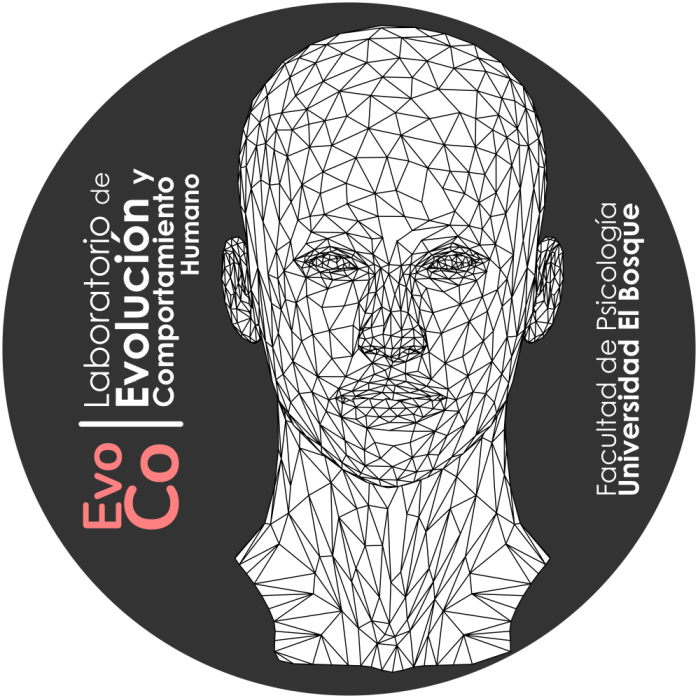
\includegraphics[width=2.3cm, height=2.3cm]{Logo_EvoCo.png}} \newline \href{https://investigaciones.unbosque.edu.co/codec}{
\includegraphics[width=2.3cm, height=2.3cm]{Logo_CODEC.png}}
\end{flushright}
\end{minipage}

\hypertarget{habilidades}{%
\section{Habilidades}\label{habilidades}}

\begin{cvskills}
  \cvskill
    {Programación}
    {\href{https://www.r-project.org/}{\textbf{R}} (avanzado: todo el procesamiento de datos, análisis, diagramas y tablas —e incluso esta HV— hechos en R)}

  \cvskill
    {Informes reproducibles}
    {Markdown/\href{https://rmarkdown.rstudio.com/}{R Markdown} (incluyendo código  \href{https://www.latex-project.org/}{{\fontfamily{cmr}\selectfont\LaTeX}} y \href{https://html.spec.whatwg.org/}{HTML}\faHtml5). Control de versiones: \href{https://git-scm.com/}{Git} \faGit* y \href{https://github.com/JDLeongomez}{GitHub} \faGithub}

  \cvskill
    {Investigación Cuantitativa}
    {Modelado estadístico, modelos de efectos mixtos, inferencia multimodelo, \textit{machine learning}}

  \cvskill
    {Software}
    {\href{https://posit.co/products/open-source/rstudio/}{RStudio}, \href{https://code.visualstudio.com/}{Visual Studio Code}, \href{https://www.fon.hum.uva.nl/praat/}{Praat}, \href{https://www.audacityteam.org/}{Audacity}, \href{https://inkscape.org/}{InkScape}, \href{https://www.zotero.org/}{Zotero}}

  \cvskill
    {Idiomas}
    {Inglés/Español}
\end{cvskills}

\hypertarget{investigaciuxf3n}{%
\section{Investigación}\label{investigaciuxf3n}}

\begin{cvskills}
  \cvskill
    {Areas de Investigacion}
    {\textbf{Voz humana • Modulación vocal • Elección de pareja • Comportamiento humano}}

  \cvskill
    {Principales Métodos de Investigación}
    {Diseños experimentales • Análisis acústico • Morfometría • Calificación de estímulos}
\end{cvskills}

\hypertarget{educaciuxf3n}{%
\section{Educación}\label{educaciuxf3n}}

\begin{cventries}
    \cventry{PhD - Psychology}{\href{https://www.stir.ac.uk/}{University of Stirling}}{Stirling, Reino Unido}{2014}{\begin{cvitems}
\item Tesis: \href{https://dspace.stir.ac.uk/handle/1893/21102}{\textbf{\textit{Contextual musicality: vocal modulation and its perception in human social interaction}}}
\item Supervisores: \href{https://www.scraigroberts.com/}{Prof. S. Craig Roberts}, y \href{https://scholar.google.com/citations?user=iDDoxVsAAAAJ}{Prof. Anthony C. Little}
\item Miembros del comité: \href{https://scholar.google.co.uk/citations?user=wxh9svQAAAAJ}{Prof. Phyllis C. Lee} (dissertation chair), y \href{https://scholar.google.com/citations?user=Qo23OGoAAAAJ}{Prof. Stuart Semple}
\end{cvitems}}
    \cventry{MSc in Evolutionary Psychology}{\href{https://www.liverpool.ac.uk/}{University of Liverpool}}{Liverpool, Reino Unido}{2009}{\begin{cvitems}
\item Supervisor: \href{https://www.scraigroberts.com/}{Prof. S. Craig Roberts}
\item Mejor desempeño general en la maestría
\end{cvitems}}
    \cventry{Licenciatura en Pedagogía Musical}{\href{https://www.upn.edu.co/}{Universidad Pedagógica Nacional}}{Bogotá, Colombia}{2006}{\begin{cvitems}
\item Trabajo de Grado: 4.90/5.00
\end{cvitems}}
\end{cventries}

\hypertarget{educaciuxf3n-complementaria-relevante}{%
\section{Educación complementaria
relevante}\label{educaciuxf3n-complementaria-relevante}}

\begin{cventries}
    \cventry{Practical Machine Learning}{Johns Hopkins University}{Coursera (MOOC platform)}{2021}{\begin{cvitems}
\item Promedio: 97/100 (ver \href{https://www.coursera.org/account/accomplishments/verify/DC7ULMJ3CZWM}{certificado})
\end{cvitems}}
    \cventry{Statistical Programming in R and Linear Mixed Models}{University of Dundee}{Dundee, Reino Unido}{2012}{}\vspace{-4.0mm}
\end{cventries}

\hypertarget{experiencia-laboral}{%
\section{Experiencia Laboral}\label{experiencia-laboral}}

\begin{cventries}
    \cventry{Profesor Asociado}{\href{https://www.unbosque.edu.co/}{Universidad El Bosque}}{Bogotá, Colombia}{Abr. 2019 - Actualmente}{\begin{cvitems}
\item Investigador en \href{https://jdleongomez.info/es/team/}{\textit{\textbf{EvoCo}: Laboratorio de Evolución y Comportamiento Humano}}
\item Líder del grupo de investigación \href{https://investigaciones.unbosque.edu.co/codec}{\textit{\textbf{CODEC}: Ciencias Cognitivas y del Comportamiento}} (desde 2016)
\item \href{https://asesores-psic.netlify.app/}{Asesor metodológico y estadístico} para proyectos de investigación de posgrado y profesores de la Facultad
\item Supervisión de una variedad de proyectos de investigación de pregrado asociados con psicología y biología
\item Miembro del Comité de Investigación
\item Miembro del Comité Asesor de Asuntos Éticos
\end{cvitems}}
    \cventry{Profesor Asistente}{\href{https://www.unbosque.edu.co/}{Universidad El Bosque}}{Bogotá, Colombia}{Ene. 2015 - Abr. 2019}{\begin{cvitems}
\item Investigador en \href{https://jdleongomez.info/es/team/}{\textit{\textbf{EvoCo}: Laboratorio de Evolución y Comportamiento Humano}}
\item Líder del grupo de investigación \href{https://investigaciones.unbosque.edu.co/codec}{\textit{\textbf{CODEC}: Ciencias Cognitivas y del Comportamiento}} (desde 2016)
\item \href{https://asesores-psic.netlify.app/}{Asesor metodológico y estadístico} para proyectos de investigación de posgrado y profesores de la Facultad
\item Organizador de la serie de conferencias semanales Café Nerd de la Facultad de Psicología (2016-2017)
\item Supervisión de una variedad de proyectos de investigación de pregrado asociados con psicología y biología
\item Estancia posdoctoral (2018-2019)
\item Co-supervisión de estudiantes de doctorado: \href{https://www.researchgate.net/profile/Milena-Vasquez-Amezquita}{Milena Vásquez-Amézquita} (PhD en Neurociencia, Universidad de Valencia, España - 2015-2018)
\item Co-supervisión de estudiantes de doctorado: Francisco Javier Flores  (Professional Doctorate in Counselling Psychology, University of East London, Reino Unido – 2016-2018)
\end{cvitems}}
    \cventry{Profesor Catedrático}{\href{https://www.unisabana.edu.co/}{Universidad de La Sabana}}{Chia, Colombia}{Ene. 2015 - Dic. 2016}{\begin{cvitems}
\item Docencia y supervisión de proyectos de investigación
\end{cvitems}}
    \cventry{Asistente de Enseñanza}{\href{https://www.stir.ac.uk/}{University of Stirling}}{Stirling, Reino Unido}{2011 - 2014}{\begin{cvitems}
\item Supervisión de un proyecto de investigación de maestría (Evolutionary Psychology MSc)
\item Calificación y asesoramiento estadístico a estudiantes de maestría
\end{cvitems}}
    \cventry{Profesor Auxiliar}{\href{https://www.upn.edu.co/}{Universidad Pedagógica Nacional}}{Bogotá, Colombia}{2010}{\begin{cvitems}
\item Miembro del Comité de Investigación
\item Supervisión de proyectos de investigación
\end{cvitems}}
\end{cventries}

\hypertarget{experiencia-docente}{%
\section{Experiencia Docente}\label{experiencia-docente}}

\begin{cventries}
    \cventry{Profesor Asociado}{\href{https://www.unbosque.edu.co/}{Universidad El Bosque}}{Bogotá, Colombia}{2019}{\begin{cvitems}
\item Métodos cuantitativos II (Maestría en Psicología) (2019)
\end{cvitems}}
    \cventry{Profesor Asistente}{\href{https://www.unbosque.edu.co/}{Universidad El Bosque}}{Bogotá, Colombia}{2015 - 2018}{\begin{cvitems}
\item Métodos cuantitativos II (Maestría en Psicología) (2017-2018)
\item Métodos cuantitativos I (Maestría en Psicología) (2017)
\item Taller Proyecto de Grado I (2018)
\item Fuentes y estilos de documentación en psicología (2015)
\end{cvitems}}
    \cventry{Profesor Catedrático}{\href{https://www.unisabana.edu.co/}{Universidad de La Sabana}}{Chia, Colombia}{2015 - 2016}{\begin{cvitems}
\item Evolución y desarrollo de la comunicación vocal: canciones, moda y lenguaje (2016)
\item Estadística inferencial (2015 - 2016)
\item Estadística descriptiva (2015 - 2016)
\end{cvitems}}
    \cventry{Adistente de Enseñanza}{\href{https://www.stir.ac.uk/}{University of Stirling}}{Stirling, Reino Unido}{2012 - 2014}{\begin{cvitems}
\item Comportamiento animal (cátedra de comunicación vocal) (2012)
\item Métodos cuantitativos (Maestría en psicología: varias conferencias, supervisión práctica, enseñanza individualizada) (2012-2014)
\item Módulo de Cognición (liderando proyectos de investigación en psicoacústica) (2012-2014)
\end{cvitems}}
    \cventry{Profesor Auxiliar}{\href{https://www.upn.edu.co/}{Universidad Pedagógica Nacional}}{Bogotá, Colombia}{2010}{\begin{cvitems}
\item Proyecto de investigación I (2010)
\item Laboratorio de investigación II (2010)
\end{cvitems}}
\end{cventries}

\hypertarget{becas-premios-y-honores}{%
\section{Becas, Premios y Honores}\label{becas-premios-y-honores}}

\begin{cventries}
    \cventry{IX Convocatoria de Estímulos a la Excelencia}{\href{https://www.unbosque.edu.co/}{Universidad El Bosque}}{Bogotá, Colombia}{Dic. 2022}{\begin{cvitems}
\item COP\$10.000.000
\end{cvitems}}
    \cventry{Economics Prize}{\href{https://improbable.com/ig/about-the-ig-nobel-prizes/}{Ig Nobel Prize}}{Cambridge, MA, EE.UU.}{Sep. 2020}{\begin{cvitems}
\item Por ‘tratar de cuantificar la relación entre la desigualdad de ingresos nacionales en diferentes países y la cantidad promedio de besos boca a boca’ (\href{https://doi.org/10.1038/s41598-019-43267-7}{Watkins, et al., 2019})
\end{cvitems}}
    \cventry{VIII Convocatoria de Estímulos a la Excelencia}{\href{https://www.unbosque.edu.co/}{Universidad El Bosque}}{Bogotá, Colombia}{Dic. 2019}{\begin{cvitems}
\item COP\$7.000.000
\end{cvitems}}
    \cventry{VII Convocatoria de Estímulos a la Excelencia}{\href{https://www.unbosque.edu.co/}{Universidad El Bosque}}{Bogotá, Colombia}{Dic. 2018}{\begin{cvitems}
\item COP\$5.000.000
\end{cvitems}}
    \cventry{VI Convocatoria de Estímulos a la Excelencia}{\href{https://www.unbosque.edu.co/}{Universidad El Bosque}}{Bogotá, Colombia}{Dic. 2017}{\begin{cvitems}
\item COP\$5.000.000
\end{cvitems}}
    \cventry{Grindley Grants}{\href{https://eps.ac.uk/}{Experimental Psychology Society}}{Canterbury, Reino Unido}{Sep. 2014}{}\vspace{-4.0mm}
    \cventry{Becas Francisco José de Caldas}{\href{https://minciencias.gov.co/}{Minciencias}}{Bogotá, Colombia}{Oct. 2010 - Oct. 2014}{}\vspace{-4.0mm}
    \cventry{Annual Prize in Evolutionary Psychology}{\href{https://www.liverpool.ac.uk/life-sciences/}{School of Life Sciences} – University of Liverpool}{Liverpool, Reino Unido}{Oct. 2009}{\begin{cvitems}
\item Mejor desempeño general en la maestría
\end{cvitems}}
    \cventry{University of Liverpool International Scholarship}{\href{https://www.liverpool.ac.uk/}{University of Liverpool}}{Liverpool, Reino Unido}{Sep. 2008 - Sep. 2009}{}\vspace{-4.0mm}
    \cventry{Programa Crédito-Beca}{\href{https://www.colfuturo.org/}{Colfuturo}}{Bogotá, Colombia}{Sep. 2008 - Sep. 2009}{}\vspace{-4.0mm}
\end{cventries}

\hypertarget{subvenciones}{%
\section{Subvenciones}\label{subvenciones}}

\begin{cventries}
    \cventry{\href{https://minciencias.gov.co/convocatorias/investigacion/convocatoria-programa-estancias-postdoctorales-beneficiarios-colciencias}{Convocatoria programa de Estancias Postdoctorales beneficiarios Colciencias 2017}}{\href{https://minciencias.gov.co/}{Minciencias}}{Bogota, Colombia}{Ene. 2018 - Ene. 2019}{\begin{cvitems}
\item Proyecto: Señales perceptibles de salud física y mental en rostros, voces y olores corporales, y su relación con niveles hormonales
\item COP\$84.000.000
\end{cvitems}}
    \cventry{IX \href{https://www.unbosque.edu.co/investigaciones/convocatorias-investigacion}{Convocatoria Interna para la Financiación de Proyectos de Investigación}, 2017}{\href{https://www.unbosque.edu.co/}{Universidad El Bosque}}{Bogota, Colombia}{Ene. 2018 - Dic. 2021}{\begin{cvitems}
\item Proyecto: Señales perceptibles de salud física y mental en rostros, voces y olores corporales, y su relación con niveles hormonales
\item COP\$136.586.537
\end{cvitems}}
    \cventry{VIII \href{https://www.unbosque.edu.co/investigaciones/convocatorias-investigacion}{Convocatoria Interna para la Financiación de Proyectos de Investigación}, 2016}{\href{https://www.unbosque.edu.co/}{Universidad El Bosque}}{Bogota, Colombia}{Ene. 2017 - Dic. 2020}{\begin{cvitems}
\item Proyecto: Efecto de señales estáticas evolutivamente relevantes (sexo, dominancia y atractivo) en el procesamiento cortical de rostros humanos
\item COP\$80.000.000
\end{cvitems}}
    \cventry{VII \href{https://www.unbosque.edu.co/investigaciones/convocatorias-investigacion}{Convocatoria Interna para la Financiación de Proyectos de Investigación}, 2015}{\href{https://www.unbosque.edu.co/}{Universidad El Bosque}}{Bogota, Colombia}{Ene. 2016 - Dic. 2019}{\begin{cvitems}
\item Proyecto: Efectos de los niveles hormonales, masculinidad y feminidad, en la discriminación tonal en hombres y mujeres
\item COP\$13.000.000
\end{cvitems}}
\end{cventries}

\hypertarget{publicaciones}{%
\section{Publicaciones}\label{publicaciones}}

\hypertarget{section}{%
\subsection{\texorpdfstring{\textbf{Artículos y Trabajos Publicados}}{}}\label{section}}

\begingroup
\footnotesize
\setlength{\parindent}{-0.5in}
\setlength{\leftskip}{0.5in}

Martínez, C. A., \& \textbf{Leongómez, J. D.} (in press). Dehumanizing
framing effects on agency, punishment, and re-socialization attributions
towards ex-perpetrators in post-conflict. \emph{Peace and Conflict:
Journal of Peace Psychology}.

Vásquez-Amézquita, M., \textbf{Leongómez, J. D.}, Salvador, A., \& Seto,
M. C. (2023). What can the eyes tell us about atypical sexual
preferences as a function of sex and age? Linking eye movements with
child-related chronophilias. \emph{Forensic Sciences Research, 8}, 5-15.
\url{https://doi.org/10.1093/fsr/owad009}

Terry, J., Ross, R. M., Nagy, T., \ldots, \textbf{Leongómez, J. D.},
\ldots, \& Field, A. P. (2023). Data from an international multi-centre
study of statistics and mathematics anxieties and related variables in
university students (the SMARVUS dataset). \emph{Journal of Open
Psychology Data, 11}(1). \url{https://doi.org/10.5334/jopd.80}

\textbf{Leongómez, J. D.}, Havlíček, J., \& Roberts, S. C. (2022).
Musicality in human vocal communication: An evolutionary perspective.
\emph{Philosophical Transactions of the Royal Society B: Biological
Sciences, 377}, 20200391. \url{https://doi.org/10.1098/rstb.2020.0391}

Santamaría-García, H., Burgaleta, M., Legaz, A., Flichtentrei, D.,
Cordoba-Delgado, M., Molina, J., Linares, J., Montealegre, J.,
Castelblanco Toro, S., Schulte, M., Paramo, J., Mondragón, I.,
\textbf{Leongómez, J. D.}, Salamone, P., González‑Pacheco, J., Baez, S.,
\& Ibañez, A.(2022). The price of prosociality in pandemic times.
\emph{Humanities and Social Sciences Communications, 9}, 15.
\url{https://doi.org/10.1057/s41599-021-01022-2}

Vásquez-Amézquita, M., Salvador, A., \& \textbf{Leongómez, J. D.}
(2022). Is digit ratio (2D:4D) different between sexual and non-sexual
offenders, and non-offending men? Study of a Colombian sample {[}Existen
diferencias en la ratio 2D:4D entre delincuentes sexuales y no sexuales,
y hombres no delincuentes? Un estudio en una muestra colombiana{]}.
\emph{Interdisciplinaria. Revista de Psicología y Ciencias Afines,
39}(1), 127--141. \url{https://doi.org/10.16888/interd.2022.39.1.8}

Watkins, C., Bovet, J., Fernandez, A. M., \textbf{Leongómez, J. D.},
Zelazniewicz, A., Correa Varella, M. A., \& Wagstaff, D. (2022). Men say
`I love you' before women do: Robust across several countries.
\emph{Journal of Social and Personal Relationships, 39}(7), 2134--2153.
\url{https://doi.org/10.1177/02654075221075264}

Fiala, V., Třebický, V., Pazhoohi, F., \textbf{Leongómez, J. D.},
Tureček, P., Saribay, S. A., \ldots{} Kleisner, K. (2021). Facial
attractiveness and preference of sexual dimorphism: A comparison across
five populations. \emph{Evolutionary Human Sciences, 3}, e38.
\url{https://doi.org/10.1017/ehs.2021.33}

Jones, B. C., DeBruine, L. M., Flake, J. K., \ldots,
\textbf{Leongómez, J. D.}, \ldots, \& Chartier, C. R. (2021). To which
world regions does the valence-dominance model of social perception
apply? \emph{Nature Human Behaviour, 5}, 159--169.
\url{https://doi.org/10.1038/s41562-020-01007-2}

Kleisner, K., \textbf{Leongómez, J. D.}, Pisanski, K., Fiala, V.,
Cornec, C., Groyecka, A., \ldots{} Akoko, R. M. (2021). Predicting
strength from aggressive vocalisations versus speech in African bushland
and urban communities. \emph{Philosophical Transactions of the Royal
Society B: Biological Sciences, 376}, 20200403.
\url{https://doi.org/10.1098/rstb.2020.0403}

Kleisner, K., Tureček, P., Roberts, S. C., Havlíček, J., Valentova, J.
V., Akoko, R. M., \textbf{Leongómez, J. D.}, Apostol, S., Varella, M. A.
C., \& Saribay, S. A. (2021). How and why patterns of sexual dimorphism
in human faces vary across the world. \emph{Scientific Reports, 11},
5978. \url{https://doi.org/10.1038/s41598-021-85402-3}

\textbf{Leongómez, J. D.}, Pisanski, K., Reby, D., Sauter, D., Lavan,
N., Perlman, M., \& Varella Valentova, J. (2021). Voice modulation: From
origin and mechanism to social impact. \emph{Philosophical Transactions
of the Royal Society B: Biological Sciences, 376}, 20200386.
\url{https://doi.org/10.1098/rstb.2020.0386}

\textbf{Leongómez, J. D.}, Sánchez, O. R., Vásquez-Amézquita, M., \&
Roberts, S. C. (2021). Contextualising courtship: Exploring male body
odour effects on vocal modulation. \emph{Behavioural Processes, 193},
104531. \url{https://doi.org/10.1016/j.beproc.2021.104531}

\textbf{Leongómez, J. D.}, Sánchez, O. R., Vásquez-Amézquita, M.,
Valderrama, E., Castellanos-Chacón, A., Morales-Sánchez, L., \ldots{}
González-Santoyo, I. (2020). Self-reported health is related to body
height and waist circumference in rural indigenous and urbanised
Latin-American populations. \emph{Scientific Reports, 10}, 4391.
\url{https://doi.org/10.1038/s41598-020-61289-4}

Bonilla, F. M., \& \textbf{Leongómez, J. D.} (2019). Efectos de la
expresión emocional y de la orientación del rostro sobre las respuestas
conductuales y el componente N170. \emph{Psychologia, 13}(2), 95--106.
\url{https://doi.org/10.21500/19002386.3473}

Vásquez Amézquita, M., \textbf{Leongómez, J. D.}, Seto, M. C., \&
Salvador, A. (2019). Differences in visual attention patterns to
sexually mature and immature stimuli between heterosexual sexual
offenders, nonsexual pffenders, and nonoffending men. \emph{Journal of
Sex Research, 56}(2), 213--228.
\url{https://doi.org/10.1080/00224499.2018.1511965}

Vásquez-Amézquita, M., \textbf{Leongómez, J. D.}, Seto, M. C., Bonilla,
F. M., Rodríguez-Padilla, A., \& Salvador, A. (2019). Visual attention
patterns differ in gynephilic and androphilic men and women depending on
age and gender of targets. \emph{Journal of Sex Research, 56}(1),
85--101. \url{https://doi.org/10.1080/00224499.2017.1372353}

Watkins, C. D., \textbf{Leongómez, J. D.}, Bovet, J., Żelaźniewicz, A.,
Korbmacher, M., Corrêa Varella, M. A., \ldots{} Bolgan, S. (2019).
National income inequality predicts cultural variation in mouth to mouth
kissing. \emph{Scientific Reports, 9}, 6698.
\url{https://doi.org/10.1038/s41598-019-43267-7}

Culpepper, P. D., Havlíček, J., \textbf{Leongómez, J. D.}, \& Roberts,
S. C. (2018). Visually activating pathogen disgust: A new instrument for
studying the behavioral immune system. \emph{Frontiers in Psychology,
9}, 1397. \url{https://doi.org/10.3389/fpsyg.2018.01397}

Danel, D. P., Valentova, J. V., Sánchez, O. R.,
\textbf{Leongómez, J. D.}, Corrêa Varella, M. A., \& Kleisner, K.
(2018). A cross-cultural study of sex-typicality and averageness:
Correlation between frontal and lateral measures of human faces.
\emph{American Journal of Human Biology, 30}(5), e23147.
\url{https://doi.org/10.1002/ajhb.23147}

Vásquez-Amézquita, M., \textbf{Leongómez, J. D.}, Seto, M. C., Bonilla,
F. M., Rodríguez-Padilla, A., \& Salvador, A. (2018). No relation
between digit ratio (2D:4D) and visual attention patterns to sexually
preferred and non-preferred stimuli. \emph{Personality and Individual
Differences, 120}, 151--158.
\url{https://doi.org/10.1016/j.paid.2017.08.022}

Bonilla, F. M., \& \textbf{Leongómez, J. D.} (2017). Efectos en la
amplitud y la latencia del componente N170 ante la presentación de
rostros emocionales de ira y miedo. \emph{Psychologia, 11}(1), 39--48.
\url{https://doi.org/10.21500/19002386.3100}

\textbf{Leongómez, J. D.}, Mileva, V. R., Little, A. C., \& Roberts, S.
C. (2017). Perceived differences in social status between speaker and
listener affect the speaker's vocal characteristics. \emph{PLOS One,
12}(6), e0179407. \url{https://doi.org/10.1371/journal.pone.0179407}

Cobey, K. D., Nicholls, M., \textbf{Leongómez, J. D.}, \& Roberts, S. C.
(2015). Self-reported dominance in women: Associations with hormonal
contraceptive use, relationship status, and testosterone. \emph{Adaptive
Human Behavior and Physiology, 1}(4), 449--459.
\url{https://doi.org/10.1007/s40750-015-0022-8}

\textbf{Leongómez, J. D.} (2015). La música como objeto de estudio
científico: consideraciones en torno a la musicalidad y el origen de la
música. \emph{(Pensamiento), (Palabra) y Obra, 13}, 77--86.
\url{https://doi.org/10.17227/2011804X.15PPO77.86}

\textbf{Leongómez, J. D.} (2014). \emph{Contextual musicality: vocal
modulation and its perception in human social interaction} {[}PhD,
University of Stirling{]}. \url{http://hdl.handle.net/1893/21102}

\textbf{Leongómez, J. D.}, Binter, J., Kubicová, L., Stolařová, P.,
Klapilová, K., Havlíček, J., \& Roberts, S. C. (2014). Vocal modulation
during courtship increases proceptivity even in naive listeners.
\emph{Evolution and Human Behavior, 35}(6), 489--496.
\url{https://doi.org/10.1016/j.evolhumbehav.2014.06.008}

Binter, J., \textbf{Leongómez, J. D.}, Moyano, N., Valentova, J., Jouza,
L., \& Klapilová, K. (2012). Sex differences in the incidence of sexual
fantasies focused on evolutionary relevant objects. \emph{Anthropologie,
50}(1), 83--93.

Ferdenzi, C., Lemaître, J.-F., \textbf{Leongómez, J. D.}, \& Roberts, S.
C. (2011). Digit ratio (2D:4D) predicts facial, but not voice or body
odour, attractiveness in men. \emph{Proceedings of the Royal Society B:
Biological Sciences, 278}(1724), 3551--3557.
\url{https://doi.org/10.1098/rspb.2011.0544}

\textbf{Leongómez, J. D.} (2009). \emph{Variation of pitch and loudness
range of human voice in response to intra- and inter-sexual stimuli}
{[}MSc{]}. University of Liverpool.

\textbf{Leongómez, J. D.} (2008). El origen no humano de la música.
\emph{(Pensamiento), (Palabra) y Obra, 1}, 87--97.
\url{https://revistas.pedagogica.edu.co/index.php/revistafba/article/view/50}

\endgroup

\hypertarget{section-1}{%
\subsection{\texorpdfstring{\textbf{\textit{Preprints} y Artículos en Revisión}}{}}\label{section-1}}

\begingroup
\footnotesize
\setlength{\parindent}{-0.5in}
\setlength{\leftskip}{0.5in}

Hadavi, S., Kuroda, J., Shimozono, T., \textbf{Leongómez, J. D.}, \&
Savage, P. E. (2023). Cross-cultural relationships between music,
emotion, and visual imagery: A comparative study of Iran, Canada, and
Japan {[}Stage 1 Registered Report{]}. \emph{PsyArXiv}.
\url{https://doi.org/10.31234/osf.io/26yg5}

Kleisner, K., Tureček, P., Saribay, S. A., Pavlovič, O.,
\textbf{Leongómez, J. D.}, Roberts, S. C., Havlíček, J., Valentova, J.
V., Apostol, S., Akoko, R. M., \& Varella, M. A. C. (submitted).
Distinctiveness and femininity, not symmetry and masculinity, affect
facial attractiveness across the world. \emph{Evolution and Human
Behavior}

\endgroup

\hypertarget{section-2}{%
\subsection{\texorpdfstring{\textbf{Articulos de Divulgacion}}{}}\label{section-2}}

\begingroup
\footnotesize
\setlength{\parindent}{-0.5in}
\setlength{\leftskip}{0.5in}

\textbf{Leongómez, J. D.} (2023). Meta-análisis de correlaciones y
meta-regresión en R: Guía práctica. \emph{MetaArXiv}.
\url{https://doi.org/10.31222/osf.io/yaxd4}

\textbf{Leongómez, J. D.} (2020). Análisis de poder estadístico y
cálculo de tamaño de muestra en R: Guía práctica. \emph{Zenodo}.
\url{https://doi.org/10.5281/zenodo.3988776}

Mileva, V. R., \& \textbf{Leongómez, J. D.} (2018). Want to know if your
partner's cheating on you? Just listen to their voice. \emph{The
Conversation}.
\url{https://theconversation.com/want-to-know-if-your-partners-cheating-on-you-just-listen-to-their-voice-92387}

Mileva, V. R., \& \textbf{Leongómez, J. D.} (2017). We change our voice
when we talk to high-status people, shows new study. \emph{The
Conversation}.
\url{https://theconversation.com/we-change-our-voice-when-we-talk-to-high-status-people-shows-new-study-80053}

\endgroup

\hypertarget{investigaciuxf3n-abierta-canal-de-youtube}{%
\section{Investigación Abierta (canal de
YouTube)}\label{investigaciuxf3n-abierta-canal-de-youtube}}

\begin{minipage}[c]{0.15\linewidth}
\href{https://www.youtube.com/@InvestigacionAbierta}{
\includegraphics[width=2.3cm, height=2.3cm]{Logo_IA.png}}
\end{minipage} \begin{minipage}[c]{0.85\linewidth}
\textcolor{red}{\faYoutube} \href{https://www.youtube.com/@InvestigacionAbierta}{Investigación Abierta} es un canal de YouTube donde publico videos y tutoriales acerca de métodos y buenas prácticas de investigación, estadística y ciencia abierta, así como algunos programas útiles de código abierto.
\end{minipage}

\begingroup
\footnotesize
\setlength{\parindent}{-0.5in}
\setlength{\leftskip}{0.5in}

\textbf{Leongómez, J. D.} {[}Investigación Abierta{]}. (2021).
\emph{Hacer meta-análisis en jamovi es muy fácil} {[}Video{]}. YouTube.
\url{https://jdleongomez.info/en/post/meta/}

\textbf{Leongómez, J. D.} {[}Investigación Abierta{]}. (2020).
\emph{Poder estadístico y tamaño de muestra en R} {[}3 Videos{]}.
YouTube. \url{https://jdleongomez.info/en/post/power/}

\textbf{Leongómez, J. D.} {[}Investigación Abierta{]}. (2020).
\emph{¿Qué es un valor p? Te lo puedo mostrar gráficamente y con
simulaciones} {[}Video{]}. YouTube.
\url{https://jdleongomez.info/en/post/pvalue/}

\textbf{Leongómez, J. D.} {[}Investigación Abierta{]}. (2020).
\emph{Introducción a jamovi} {[}2 Videos{]}. YouTube.
\url{https://jdleongomez.info/en/post/jamovi/}

\textbf{Leongómez, J. D.} {[}Investigación Abierta{]}. (2020).
\emph{Introducción a OBS Studio} {[}Video{]}. YouTube.
\url{https://jdleongomez.info/en/post/obs/}

\endgroup

\hypertarget{shiny-apps}{%
\section{Shiny Apps}\label{shiny-apps}}

\begin{minipage}[c]{0.10\linewidth}
\href{https://jdleongomez.info/es/#shiny}{
\includegraphics[width=1.5cm, height=1.74cm]{shiny_hex.png}}
\end{minipage} \begin{minipage}[c]{0.90\linewidth}
He creado algunas, pequeñas aplicaciones públicas con \href{https://shiny.posit.co/}{Shiny} en R, sobre todo por diversión. Aunque todavía estoy aprendiendo, en esta sección hay algunos ejemplos.
\end{minipage}

\begingroup
\footnotesize
\setlength{\parindent}{-0.5in}
\setlength{\leftskip}{0.5in}

\textbf{Leongómez, J. D.} (2023). \textbf{\emph{PowerSimulate}}
{[}Colección de aplicaciones{]}.
\url{https://shiny.jdl-svr.lat/PowerSimulate/}

\textbf{Leongómez, J. D.} (2023). \emph{\textbf{ScolarlyOutput}: Crea y
exporta un gráfico completo de tu perfil de Google académico} (Versión
1.0.0) {[}Software{]}.
\href{https://github.com/JDLeongomez/ScholarlyOutput_ES}{https://doi.org/10.5281/zenodo.8060475}

\textbf{Leongómez, J. D.} (2021). \emph{\textbf{ProbDnD}: Probabilidad
de obtener un valor en DnD, combinando múltiples dados y un modificador}
{[}Software{]}. \url{https://github.com/JDLeongomez/ProbDnD}

\endgroup

\hypertarget{presentaciones-en-conferencias-puxf3sters-y-talleress}{%
\section{Presentaciones en Conferencias, Pósters y
Talleress}\label{presentaciones-en-conferencias-puxf3sters-y-talleress}}

\begingroup
\footnotesize
\setlength{\parindent}{-0.5in}
\setlength{\leftskip}{0.5in}

\textbf{Leongómez, J. D.} (2023, agosto). \emph{Potenciando tus
conclusiones: Explorando la vital importancia del poder estadístico y el
tamaño de muestra en la inferencia confiable}. Presentación invitada al
XXIX Congreso Institucional de Investigaciones (Universidad El Bosque),
Bogotá, Colombia.
\url{https://investigaciones.unbosque.edu.co/s/D-00730__ViceInvestigaciones__-agenda-Congreso-Institucional-links-1.pdf}

\textbf{Leongómez, J. D.} (2023, julio). \emph{From data to knowledge:
Conducting meta-analyses of correlations and t-tests}. Taller invitado
presentado en el Summer Institute 2023 de of the International Society
for Human Ethology (ISHE), Universidade Federal de Pernambuco, Recife,
Brasil. \url{https://ishe.org/wp-content/uploads/2023/07/BoA_v06_km.pdf}
(ver
\href{https://jdleongomez.info/es/files/Cert_ISHE_2023.pdf}{certificado})

\textbf{Leongómez, J. D.} (2023, julio). \emph{Ensuring reliable
results: Power analysis and sample size estimation in behavioural
research}. Taller invitado presentado en el Summer Institute 2023 de of
the International Society for Human Ethology (ISHE), Universidade
Federal de Pernambuco, Recife, Brasil.
\url{https://ishe.org/wp-content/uploads/2023/07/BoA_v06_km.pdf} (ver
\href{https://jdleongomez.info/es/files/Cert_ISHE_2023.pdf}{certificado})

\textbf{Leongómez, J. D.}, Havlíček, J., \& Roberts, S.C. (2022,
octubre). \emph{Musicality in human vocal communication}. Artículo
presentado como parte del simposio The Evolution of Human Musicality en
el 4th Brazilian Meeting on Evolution of Human Behavior (Universidad de
São Paulo), São Paulo, Brasil. \url{https://youtu.be/gK_rl0r4nfs?t=9662}

\textbf{Leongómez, J. D.} (2022, octubre). \emph{Sesión presencial de
jamovi}. Taller para el Plan de formación en investigación de la
Vicerrectoría de Investigaciones (Universidad El Bosque), Bogotá,
Colombia.

\textbf{Leongómez, J. D.} (2022, septiembre). \emph{Introducción a
jamovi: Alternativa moderna, gratuita y de código abierto para la
realización de análisis estadísticos}. Presentación organizada como
parte del Plan de formación en investigación de la Vicerrectoría de
Investigaciones (Universidad El Bosque), Bogotá, Colombia.
\url{https://investigaciones.unbosque.edu.co/eventos/cuestioneseticas-jjnlm-92bkj-n249w-hbnhl-6tpj4-pm22x-8m3yh-645tt-gw59h-xwc6x-d9sgw-6fzel-hm6dd-2wrls-569m2-8zns8-rg363}

\textbf{Leongómez, J. D.} (2022, agosto). \emph{Más allá del Open
Access: Necesidad de una Ciencia Abierta integral para enfrentar las
implicaciones de la naturalización de malas prácticas y la crisis de la
replicación}. Presentación organizada como parte del Plan de formación
en investigación de la Vicerrectoría de Investigaciones (Universidad El
Bosque), Bogotá, Colombia.
\url{https://investigaciones.unbosque.edu.co/eventos/cuestioneseticas-jjnlm-92bkj-n249w-hbnhl-6tpj4-pm22x-8m3yh-645tt-gw59h-xwc6x-d9sgw-6fzel-hm6dd-2wrls-569m2-8zns8}

\textbf{Leongómez, J. D.} (2022, abril). \emph{¿Qué tan confiable es la
literatura científica? Ciencia abierta como estrategia para enfrentar
las implicaciones de la naturalización de malas prácticas y la crisis de
la replicación}. Presentación organizada por la Unidad de
Investigaciones de la Facultad de Psicología (Universidad El Bosque),
Bogotá, Colombia. \url{https://youtu.be/Fl98MoBqSaI}

\textbf{Leongómez, J. D.} (2020, noviembre). \emph{¿Cuántos
participantes necesito? Análisis de poder estadístico y cálculo de
tamaño de muestra en R}. Taller para el Congreso Internacional de
Neurociencias: Cerebro y Comportamiento en Tiempos de COVID-19
(Universidad El Bosque, Universidad de los Andes), Bogotá, Colombia.
\url{https://youtu.be/tVB9sh5ZFH0}

\textbf{Leongómez, J. D.} \& Sánchez, O. R. (2019, septiembre).
\emph{Asociación entre altura y circunferencia de cintura con salud en
poblaciones rurales indígenas y urbanas en América Latina}. Artículo
presentado en el XXV Congreso Institucional de Investigaciones
(Universidad El Bosque), Bogotá, Colombia.

\textbf{Leongómez, J. D.}, Sánchez, O.R., Vásquez-Amézquita, M.,
Valderrama, E., Castellanos-Chacón, A., Morales-Sánchez, L., Nieto, J.,
\& González-Santoyo, I. (2019, agosto). \emph{Self-reported Health is
Related to Body Height and Waist Circumference in Rural Indigenous and
Urbanised Latin-American Populations}. Artículo y póster presentados en
el VII Summer Institute of the International Society for Human Ethology
(ISHE), Zadar, Croatia. Póster:
\url{https://jdleongomez.info/en/publication/leongomez2020/PosterA0.pdf}

\textbf{Leongómez, J. D.} (2019, juio). \emph{Diseños Experimentales}.
Taller para la Vicerrectoría de Investigaciones (Universidad El Bosque),
Bogotá, Colombia.

\textbf{Leongómez, J. D.}, Murray, A.K., \& Roberts, S.C. (2018,
septiembre). \emph{Contextualising courtship: Male body odour effects on
vocal modulation}. Artículo presentado en el XXIV Biannual Conference
for Human Ethology (ISHE), Santiago, Chile.

\textbf{Leongómez, J. D.} (2017, septiembre). \emph{Efectos de los
niveles hormonales, masculinidad y feminidad, en la discriminación tonal
de hombres y mujeres.}. Artículo presentado en el XXIII Congreso
Institucional de Investigaciones (Universidad El Bosque), Bogotá,
Colombia.

\textbf{Leongómez, J. D.} (2017, agosto). \emph{The sound of seduction:
Vocal modulations and their effects during courtship}. Sesión plenaria
en el 2do Simposio de Neurociencias, Cognición y Sociedad (Universidad
Javeriana), Bogotá, Colombia.

\textbf{Leongómez, J. D.} (2017, marzo). \emph{Is the relationship
between musical and linguistic processing a vestige of the evolutionary
origins of music?}. Sesión plenaria en el 2017 Brain Awareness Week 2017
(Universidad El Bosque), Bogotá, Colombia.

\textbf{Leongómez, J. D.}, Mileva, V.R., Little, A.C., \& Roberts, S.C.
(2016, agosto). \emph{Perceived differences in social status between
speaker and listener affect the speaker's vocal characteristics}.
Artículo presentado en el XXIII Biennial Congress On Human Ethology
(ISHE), Stirling, Reino Unido.

\textbf{Leongómez, J. D.}, Binter, J., Kubicová, L., Stolařová, P.,
Klapilová, K., Havlíček, J., \& Roberts, S.C. (2014, abril). \emph{Vocal
modulation during courtship increases proceptivity even in naive
listeners}. Artículo presentado en el European Human Behaviour and
Evolution Association (EHBEA) Annual Meeting 2014 (University of
Bristol), Bristol, Reino Unido.

\textbf{Leongómez, J. D.}, \& Roberts, S.C. (2013, abril). \emph{The
sound of sweet nothings: How men and women modulate vocal parameters in
speech directed towards attractive and unattractive individuals}.
Presentación oral para el Mind and Brain Group (University of Stirling),
Stirling, Reino Unido.

\textbf{Leongómez, J. D.}, \& Roberts, S.C. (2013, marzo). \emph{The
sound of sweet nothings: How men and women modulate vocal parameters in
speech directed towards attractive and unattractive individuals}. Póster
presentado en el European Human Behaviour and Evolution Association
(EHBEA) Annual Meeting 2013 (VU University Amsterdam), Amsterdam,
Netherlands.

\textbf{Leongómez, J. D.} (2013, marzo). \emph{Voice research techniques
using Praat}. Taller en la Facultad de Humanidades (Charles University),
Praga, República Checa.

\textbf{Leongómez, J. D.} (2013, marzo). \emph{Acoustic Communication}.
Presentación oral en el Centre for Theoretical Study, Praga, República
Checa.

\textbf{Leongómez, J. D.}, \& Roberts, S.C. (2012, mayo). \emph{The
sound of sweet nothings: How men and women modulate vocal parameters in
speech directed towards attractive and unattractive individuals}.
Presentación oral para el Group of Human Ethology (Charles University),
Praga, República Checa.

\textbf{Leongómez, J. D.} (2013, marzo). \emph{Voice research techniques
using Praat}. Taller en Scottish Universities Psychology Postgraduate
Research Training -- SUPPORT (University of Stirling), Stirling, Reino
Unido.

\textbf{Leongómez, J. D.}, \& Roberts, S.C. (2011, febrero). \emph{The
sound of sweet nothings: How men and women modulate vocal parameters in
speech directed towards attractive and unattractive individuals}.
Presentación para el Behaviour and Evolution Research Group (University
of Stirling), Stirling, Reino Unido.

\textbf{Leongómez, J. D.}, \& Roberts, S.C. (2010, diciembre).
\emph{Context-dependant modulation of vocal parameters}. Póster
presentado en el Language of Music, the Music of Language; Meeting 2:
Entrainment/Meaning (Centre for Music \& Science, University of
Cambridge), Cambridge, Reino Unido.

\endgroup

\hypertarget{eventos-cientuxedficos}{%
\section{Eventos Científicos}\label{eventos-cientuxedficos}}

\begin{cventries}
    \cventry{Presidente del Comité Científico}{CIVN2020 - Congreso Internacional de Neurociencias: Cerebro y Comportamiento en Tiempos de COVID-19}{Universidad El Bosque y Universidad de los Andes}{Nov. 25 ‑ 28, 2020}{\begin{cvitems}
\item \href{http://doi.org/10.17605/OSF.IO/5BWNX}{Memorias}
\item \href{https://www.youtube.com/@onlineinternationalcongres6942}{Canal de YouTube} (Todo el congreso disponible)
\end{cvitems}}
    \cventry{Miembro del Comité Científico}{1er Congreso Internacional Virtual ISEP}{ISEP}{May. 5 - 7, 2020}{\begin{cvitems}
\item \href{https://www.isep.es/congreso2020/\#comite}{Comité Científico}
\end{cvitems}}
\end{cventries}

\hypertarget{roles-editoriales}{%
\section{Roles Editoriales}\label{roles-editoriales}}

\begin{small}
\textbf{Nota:} Mi registro verificado como par académico y editos internacional está disponible en mi perfil de \href{https://www.webofscience.com/wos/author/record/387716}{Web of Science}.
\end{small}

\begin{cventries}
    \cventry{Recommender (editor)}{\href{https://rr.peercommunityin.org/}{PCI Registered Reports}}{Recommender}{Desde 2023}{\begin{cvitems}
\item Emisión de recomendaciones de las fases 1 y 2
\item Perfil \href{https://rr.peercommunityin.org/public/user_public_page?userId=1996}{Recommender}
\end{cvitems}}
    \cventry{Guest Editor}{\href{https://royalsocietypublishing.org/journal/rstb}{Philosophical Transactions of the Royal Society B: Biological Sciences}}{Comité Editorial invitado}{2020 - 2021}{\begin{cvitems}
\item Theme Issue \textbf{\textit{Voice modulation: from origin and mechanism to social impact}} (\href{https://royalsocietypublishing.org/toc/rstb/2021/376/1840}{\textbf{Parte 1}}, \href{https://royalsocietypublishing.org/toc/rstb/2022/377/1841}{\textbf{Parte 2}})
\item Editado por Juan David Leongómez, Katarzyna Pisanski, David Reby, Disa Sauter, Nadine Lavan, Marcus Perlman y Jaroslava Varella Valentova
\end{cvitems}}
    \cventry{Review Editor}{\href{https://www.frontiersin.org/journals/psychology}{Frontiers in Psychology}}{Equipo editorial}{2019 - Actualmente}{\begin{cvitems}
\item Specialty section on \href{https://www.frontiersin.org/journals/psychology/sections/evolutionary-psychology}{Evolutionary Psychology}
\item Perfil \href{https://loop.frontiersin.org/people/438954/overview}{Loop}
\end{cvitems}}
    \cventry{Journals Incluyen}{Par \textit{Ad Hoc}}{\textit{Journals} Internacionales}{Desde 2013}{\begin{cvitems}
\item \href{https://royalsocietypublishing.org/journal/rspb}{Proceedings of the Royal Society B: Biological Sciences}
\item \href{https://royalsocietypublishing.org/journal/rsos}{Royal Society Open Science}
\item \href{https://journals.plos.org/plosone/}{PLOS ONE}
\item \href{https://royalsocietypublishing.org/journal/rsbl}{Biology Letters}
\item \href{https://www.sciencedirect.com/journal/evolution-and-human-behavior}{Evolution and Human Behavior}
\item \href{https://www.nature.com/srep/}{Scientific Reports}
\item \href{https://www.sciencedirect.com/journal/cortex}{Cortex}
\item \href{https://www.springer.com/journal/10919/}{Journal of Nonverbal Behavior}
\item \href{https://journals.sagepub.com/home/pec}{Perception}
\item \href{https://www.tandfonline.com/journals/hbas20}{Basic and Applied Social Psychology}
\item \href{https://www.frontiersin.org/journals/psychology}{Frontiers in Psychology}
\item \href{https://journals.sagepub.com/home/evp}{Evolutionary Psychology}
\item \href{http://sumapsicologica.konradlorenz.edu.co/}{Summa Psicológica}
\item \href{https://ishe.org/human-ethology/}{Human Ethology}
\end{cvitems}}
    \cventry{Evaluación de Publicaciones}{Par Académico}{Instituciones Colombianas}{Desde 2015}{\begin{cvitems}
\item \href{https://minciencias.gov.co/}{Minciencias}
\item \href{https://unal.edu.co/}{Universidad Nacional de Colombia}
\end{cvitems}}
\end{cventries}

\hypertarget{supervisiuxf3n-de-investigaciuxf3n}{%
\section{Supervisión de
Investigación}\label{supervisiuxf3n-de-investigaciuxf3n}}

\hypertarget{section-3}{%
\subsection{\texorpdfstring{\textbf{Posgrado}}{}}\label{section-3}}

La Facultad de Psicología de la Universidad El Bosque no ofrece títulos
de investigación, y todos los cursos de nivel de maestrías son
profesionales. Debido a esto, las oportunidades de supervisar a
estudiantes de posgrado son limitadas, y la mayor parte de mi
supervisión de posgrado ha sido externa.

\begin{cventries}
    \cventry{PhD in Neuroscience}{\href{https://www.researchgate.net/profile/Milena-Vasquez-Amezquita}{Milena Vásquez-Amézquita}}{\href{https://www.uv.es/}{Universitat de València}, España}{2015 - 2018}{\begin{cvitems}
\item Tésis \textbf{\textit{(Summa Cum Laude)}}: \textit{\href{http://hdl.handle.net/10550/67639}{Preferencias sexuales típicas y atípicas según sexo y edad de los estímulos: Utilidad de la técnica de rastreo ocular} [Typical and atypical sexual preferences according to sex and age of the stimuli: Usefulness of the eye tracking technique]}
\item Supervisión conjunta con  Alicia Salvador
\end{cvitems}}
    \cventry{Professional Doctorate in Counselling Psychology}{\href{https://www.researchgate.net/profile/Francisco-Flores-14}{Francisco Javier Flores}}{\href{https://www.uel.ac.uk/}{U. of East London}, Reino Unido}{2015 - 2018}{\begin{cvitems}
\item Tésis: \textit{ What sense do people make of the functions of their ’behaviours that may be causing problems in their everyday life’? A hybrid deductive/inductive template analysis}
\item Supervisión conjunta con Lisa Chiara Fellin
\end{cvitems}}
    \cventry{Maestría en Psicología}{Adrián Acosta Guerrero}{\href{https://www.unbosque.edu.co/}{Universidad El Bosque}, Colombia}{2019 - 2020}{\begin{cvitems}
\item Trabajo de grado \textbf{\textit{(Meritorio)}}: \textit{\href{http://hdl.handle.net/20.500.12495/4416}{La voz como predictor de sintomatología asociada a depresión y ansiedad} [Voice as a predictor of symptomatology associated with depression and anxiety]}
\item Supervisión conjunta con \href{https://www.researchgate.net/profile/Milena-Vasquez-Amezquita}{Milena Vásquez-Amézquita}
\end{cvitems}}
    \cventry{Psychological Research Methods (Evolutionary Psychology) MSc}{Julia Sanz-Vidania}{\href{https://www.stir.ac.uk/}{University of Stirling}, Reino Unido}{2013 - 2014}{\begin{cvitems}
\item Trabajo de grado \textbf{\textit{(Meritorio)}}: \textit{Sexy Chat: Mate-Choice Preferences for Speech Content in the Absence of Auditory Cues}
\item Supervisión conjunta con \href{https://www.scraigroberts.com/}{S Craig Roberts}
\end{cvitems}}
\end{cventries}

\hypertarget{section-4}{%
\subsection{\texorpdfstring{\textbf{Pregrado}}{}}\label{section-4}}

Los estudiantes universitarios supervisados que figuran a continuación
proceden de distintas universidades y programas académicos. Esta lista
sólo incluye a los estudiantes de quienes fui supervisor principal u
obtuvieron mención a trabajo de grado meritorio. Adicionalmente,
actualmente estoy supervisando seis estudiantes como supervisor
principal, y he supervisado a más de 25 estudiantes como co-supervisor.

\begin{cventries}
    \cventry{Psicología}{Andrés Castellanos-Chacón}{\href{https://www.unbosque.edu.co/}{Universidad El Bosque}, Colombia}{Desde 2017}{\begin{cvitems}
\item Supevisión práctica profesional (investigación)
\item Proyecto: \textit{Señales perceptibles de salud física y mental en rostros, voces y olores corporales, y su relación con niveles hormonales}
\item \textbf{\textit{Trabajo de grado meritorio}}
\item Supervisión docente (2019 - actualmente)
\end{cvitems}}
    \cventry{Psicología}{Maria Camila Wilches y Johan Sebatián Castiblanco}{\href{https://www.unbosque.edu.co/}{Universidad El Bosque}, Colombia}{2022 - 2023}{\begin{cvitems}
\item Trabajo de grado: \textit{\href{https://youtu.be/FlZvukFqTcc}{El rol del género en la identificación de la sociosexualidad a partir de las voces}}
\end{cvitems}}
    \cventry{Psicología}{Angie Alejandra Lozano Sanjuan, Daniela Martínez Franco y Mariana Saavedra Botero}{\href{https://www.unbosque.edu.co/}{Universidad El Bosque}, Colombia}{2021 - 2022}{\begin{cvitems}
\item \textbf{\textit{Trabajo de grado meritorio}}: \textit{\href{https://youtu.be/A9xNV3BqRJw}{¿Somos capaces de detectar qué tan sociosexual es una persona a partir de su voz y/o su rostro?}}
\end{cvitems}}
    \cventry{Psicología}{John Jairo Rubio}{\href{https://www.unbosque.edu.co/}{Universidad El Bosque}, Colombia}{2021 - 2022}{\begin{cvitems}
\item Trabajo de grado: \textit{\href{https://youtu.be/G9eqxpyKF5A}{¿Existe relación entre la simetría facial y el atractivo de la voz?} }
\end{cvitems}}
    \cventry{Psicología}{Maria Daniela Martínez Luna y Juan Sebastián Preciado Ruíz}{\href{https://www.unbosque.edu.co/}{Universidad El Bosque}, Colombia}{2020 - 2021}{\begin{cvitems}
\item \textbf{\textit{Trabajo de grado meritorio}}: \textit{\href{https://youtu.be/BNNseX-PK7s}{¿Existe relación entre la sociosexualidad y la voz?}}
\end{cvitems}}
    \cventry{Psicología}{Maria Paula Moreno Rodríguez y Andrés Felipe Orozco Serrato}{\href{https://www.unbosque.edu.co/}{Universidad El Bosque}, Colombia}{2019 - 2021}{\begin{cvitems}
\item Trabajo de grado: \textit{\href{https://youtu.be/qHn87CoBEm4}{¿Existe relación entre la forma del rostro y la socio-sexualidad?}}
\end{cvitems}}
    \cventry{Psicología}{Danny Ferley Gaitan Rodríguez y Hasbleidy Gamboa Ordoñez}{\href{https://www.unbosque.edu.co/}{Universidad El Bosque}, Colombia}{2019 - 2020}{\begin{cvitems}
\item Trabajo de grado: \textit{\href{https://youtu.be/J6nUuifYjbU}{Detección de infidelidad y sociosexualidad a partir de rostros: Análisis preliminar}}
\end{cvitems}}
    \cventry{Pedagogía Musical}{Natalia Elízabeth Moreno Buitrago y Juan Felipe Pérez Ariza}{\href{https://www.upn.edu.co/}{U. Pedagógica Nacional}, Colombia}{2017 - 2019}{\begin{cvitems}
\item \textbf{\textit{Trabajo de grado meritorio}}: \textit{\href{http://hdl.handle.net/20.500.12209/10443}{Musicalidad y cohesión social: una aproximación experimental y bibliográfica desde el trabajo en equipo}}
\end{cvitems}}
    \cventry{Psicología}{Paula Andrea Betancourt Velandia y Ana Sofía Gómez Castelblanco}{\href{https://www.unbosque.edu.co/}{Universidad El Bosque}, Colombia}{2018 - 2019}{\begin{cvitems}
\item Trabajo de grado: \textit{Hombres que alcanzan voces menos agudas y con un volumen más bajo, tienden a tener más relaciones sexuales casuales}
\end{cvitems}}
    \cventry{Biología}{Maria Alejandra Abello Mozo}{\href{https://www.unbosque.edu.co/}{Universidad El Bosque}, Colombia}{2017 - 2018}{\begin{cvitems}
\item \textbf{\textit{Trabajo de grado meritorio}}: \textit{Desarrollo y evaluación de una metodología nueva para manipular las variables del atractivo, dominancia y sexo simultáneamente en fotos de caras humanas con el programa PsychoMorph}
\end{cvitems}}
    \cventry{Psicología}{Cindy Paola Moncada Gómez}{\href{https://www.unbosque.edu.co/}{Universidad El Bosque}, Colombia}{2017 - 2018}{\begin{cvitems}
\item Trabajo de grado: \textit{La voz del sexo casual: ¿las características vocales predicen la disposición al sexo sin compromiso en hombres y mujeres? A}
\end{cvitems}}
    \cventry{Psicología}{Laura Milena Estupiñan Aldana}{\href{https://www.unbosque.edu.co/}{Universidad El Bosque}, Colombia}{2017 - 2018}{\begin{cvitems}
\item Trabajo de grado: \textit{La voz del sexo casual: ¿las características vocales predicen la disposición al sexo sin compromiso en hombres y mujeres? B}
\end{cvitems}}
    \cventry{Psicología}{Vanesa Díaz Güiza}{\href{https://www.unbosque.edu.co/}{Universidad El Bosque}, Colombia}{2016 - 2018}{\begin{cvitems}
\item Trabajo de grado: \textit{La voz del sexo casual: ¿las características vocales predicen la disposición al sexo sin compromiso en hombres y mujeres? C}
\end{cvitems}}
    \cventry{Psicología}{Lina María García Hoyos}{\href{https://www.unbosque.edu.co/}{Universidad El Bosque}, Colombia}{2016 - 2018}{\begin{cvitems}
\item Trabajo de grado: \textit{¿Se puede determinar si una persona ha sido infiel a partir de su voz?}
\end{cvitems}}
    \cventry{Psicología}{Angie Liliana Pérez Rodríguez}{\href{https://www.unbosque.edu.co/}{Universidad El Bosque}, Colombia}{2016 - 2017}{\begin{cvitems}
\item Trabajo de grado: \textit{Efectos de los niveles hormonales en la discriminación tonal de mujeres}
\end{cvitems}}
    \cventry{Psicología}{Lina María Morales Sánchez}{\href{https://www.unbosque.edu.co/}{Universidad El Bosque}, Colombia}{2016 - 2017}{\begin{cvitems}
\item Trabajo de grado: \textit{Discriminación tonal predice satisfacción con pareja y su inversión parental, en hombres y mujeres}
\end{cvitems}}
    \cventry{Psicología}{Haydn Ricardo Roldán Morales}{\href{https://www.unbosque.edu.co/}{Universidad El Bosque}, Colombia}{2015 - 2016}{\begin{cvitems}
\item Trabajo de grado: \textit{El sonido de la seducción: discriminación tonal, satisfacción en pareja, y niveles hormonales en hombres}
\end{cvitems}}
\end{cventries}

\hypertarget{membresuxedas}{%
\section{Membresías}\label{membresuxedas}}

\begin{cventries}
    \cventry{\href{https://ishe.org/}{International Society for Human Ethology} (ISHE)}{}{}{2016 - Actualmente}{}\vspace{-4.0mm}
    \cventry{\href{https://www.psychologicalscience.org/}{Association for Psychological Science} (APS)}{}{}{2013 - 2020}{}\vspace{-4.0mm}
    \cventry{\href{https://www.cambridge.org/core/membership/ehbea}{European Human Behaviour and Evolution Association} (EHBEA)}{}{}{2013 - 2016}{}\vspace{-4.0mm}
\end{cventries}



\end{document}
